% !TEX program = xelatex
% 공통수학2 · Ⅲ. 함수와 그래프 · 2. 유리함수와 무리함수 · 02 무리함수 · 1/1차시
\documentclass[11pt,a4paper]{article}
\usepackage{kotex}
\usepackage{iftex}
\ifPDFTeX\else
  \setmainhangulfont{Noto Serif CJK KR}
  \setsanshangulfont{Noto Sans CJK KR}
\fi
\usepackage[margin=2.1cm]{geometry}
\usepackage{parskip}
\usepackage{enumitem}
\usepackage{array}
\usepackage{tabularx}
\usepackage{booktabs}
\usepackage{xcolor}
\usepackage{amssymb}
\usepackage{tikz}
\usepackage[most]{tcolorbox}
\usepackage{fancyhdr}
\usepackage{titlesec}

\definecolor{goldc}{HTML}{B07C22}
\definecolor{goldstrong}{HTML}{8A5F16}
\definecolor{indigoc}{HTML}{2B3B57}
\definecolor{indigosoft}{HTML}{6E82A6}
\definecolor{linec}{HTML}{D6DACB}
\definecolor{surface2}{HTML}{E4E8DC}
\definecolor{notebg}{HTML}{FBF3E3}
\definecolor{inksoft}{HTML}{52604F}

\titleformat{\section}{\normalfont\sffamily\bfseries\large\color{indigoc}}{\thesection}{0.6em}{}
\titlespacing{\section}{0pt}{16pt}{8pt}
\newtcolorbox{ideabox}{enhanced, breakable, colback=white, colframe=goldc, boxrule=0.5pt, leftrule=3pt, arc=2pt, left=10pt, right=10pt, top=8pt, bottom=8pt}
\newtcolorbox{calloutbox}{enhanced, breakable, colback=white, colframe=indigosoft, boxrule=0.5pt, leftrule=3pt, arc=2pt, left=10pt, right=10pt, top=7pt, bottom=7pt}
\newtcolorbox{notebox}{enhanced, breakable, colback=notebg, colframe=goldc, boxrule=0.5pt, leftrule=3pt, arc=2pt, left=10pt, right=10pt, top=7pt, bottom=7pt}
\newtcolorbox{answerbox}{enhanced, breakable, colback=white, colframe=linec, boxrule=0.5pt, arc=2pt, left=10pt, right=10pt, top=7pt, bottom=7pt}
\newcommand{\lessonbanner}[3]{%
  \begin{tcolorbox}[enhanced, colback=indigoc, colframe=indigoc, boxrule=0pt, arc=0pt,
    left=14pt, right=14pt, top=14pt, bottom=10pt, borderline south={2.4pt}{0pt}{goldc}, fontupper=\color{white}]
    {\sffamily\footnotesize\color{white!85!black} #1}\\[4pt]{\sffamily\bfseries\Large #2}\\[3pt]{\sffamily\small\color{white!88!black} #3}
  \end{tcolorbox}}
\pagestyle{fancy}\fancyhf{}\renewcommand{\headrulewidth}{0pt}
\fancyfoot[L]{\footnotesize\color{inksoft} 공통수학2 · 2026학년도 2학기 · 지평선고등학교}
\fancyfoot[R]{\footnotesize\color{inksoft} 교사용 지도안 -- 배포 금지}

\begin{document}
\lessonbanner{공통수학2 · Ⅲ. 함수와 그래프 · 2. 유리함수와 무리함수}{02 무리함수 --- 1/1차시}{무리함수의 뜻, 정의역, 그래프 · 교사용 지도안 (2026학년도 2학기)}
\vspace{10pt}

\noindent\begin{tabularx}{\linewidth}{@{}>{\bfseries\color{indigoc}}p{2.6cm}X@{}}
\toprule
대상 & 고1 · 2개 반 · 반당 13명 \\
차시 & 50분 (도입 10 · 전개 30 · 정리 10) \\
성취기준 & 무리함수의 뜻을 알고, 정의역을 구하며 그래프를 그릴 수 있다. \\
선행 학습 & 39$\sim$40차시 --- 유리함수의 뜻과 그래프, 14차시 --- 평행이동 \\
\bottomrule
\end{tabularx}

\section{학습 목표 \& Big Idea}
\begin{ideabox}
\textbf{\color{goldstrong}영속적 이해 (Big Idea)}\\
실수의 제곱근은 근호 안이 음수이면 존재하지 않는다. 그래서 무리함수는 근호 안의 식이 $0$ 이상이 되는 범위로만 정의역이 제한되며, 이 제한이 곧 무리함수 그래프가 `반쪽짜리 곡선'으로 나타나는 이유이다.
\vspace{4pt}
\small\color{inksoft} 핵심개념: \textbf{근호 안의 부등식} \quad\textbullet\quad 핵심개념: \textbf{평행이동} \quad\textbullet\quad 일반화: \textbf{무리함수의 그래프는 $y=\sqrt{ax}$의 평행이동이다}
\end{ideabox}
\begin{calloutbox}
\textbf{차시 학습 목표}
\begin{itemize}[leftmargin=1.4em, itemsep=2pt, topsep=4pt]
  \item 무리식과 무리함수의 뜻을 알고, 근호 안의 식이 $0$ 이상이라는 조건으로 정의역을 구할 수 있다.
  \item $y=\sqrt{a(x-p)}+q$의 그래프를 그리고, 정의역과 치역을 구할 수 있다.
\end{itemize}
\end{calloutbox}

\section{질문의 연결}
\begin{tabularx}{\linewidth}{@{}>{\bfseries\color{indigoc}\small}p{2.4cm}X@{}}
사실적 질문 & 무리함수 $y=\sqrt{ax+b}+c$의 정의역은 어떻게 구할까? \\[6pt]
개념적 질문 & 왜 근호 안의 식은 항상 $0$ 이상이어야 할까? \\[6pt]
논쟁적 질문 & ``제한이 있어야 오히려 명확해진다''는 말에 동의하는가? 무리함수의 정의역 제한을 예로 들어 생각을 나눠 보자. \\
\end{tabularx}

\section{수업 흐름}
\begin{tabularx}{\linewidth}{@{}>{\centering\arraybackslash}p{1.6cm}X>{\raggedright\arraybackslash\small}p{3.1cm}@{}}
\toprule
\textbf{단계} & \textbf{활동 \& 발문} & \textbf{ATL / VTR} \\
\midrule
\textcolor{goldstrong}{\textbf{도입}}\newline\footnotesize 10분 &
\textbf{마음공부 (2분)} --- 유무념 대조.\newline
\textbf{생각 열기 (8분)} --- 넓이가 $A$인 정사각형의 한 변의 길이는 $x=\sqrt A$. $A=9,4,1,0,-4$일 때 $x$를 구해 보며 $A<0$일 때 왜 정의할 수 없는지 토의. &
ATL: 사고(실생활 연결)\newline VTR: See-Think-Wonder \\
\addlinespace
\textcolor{goldstrong}{\textbf{전개}}\newline\footnotesize 30분 &
\textbf{무리식과 무리함수의 뜻 (8분)} --- 근호 안에 문자를 포함하고 근호를 없앨 수 없는 식이 무리식, 무리식으로 나타낸 함수가 무리함수임을 정의 $\to$ 문제 1.\newline
\textbf{정의역 구하기 (10분)} --- 근호 안의 식 $\geq0$을 만족하는 $x$의 범위가 정의역임을 확인 $\to$ 문제 2.\newline
\textbf{그래프와 평행이동 (12분)} --- $y=\sqrt{ax}$ ($a>0$: 정의역 $x\geq0$, 증가 / $a<0$: 정의역 $x\leq0$)의 그래프 $\to$ $y=\sqrt{a(x-p)}+q$는 $(p,q)$만큼 평행이동 $\to$ 문제 3, 문제 4(그래프 정보로 식 역산). &
ATT: 촉진자 역할\newline ATL: 대수적 조작·기하적 추론 \\
\addlinespace
\textcolor{goldstrong}{\textbf{정리}}\newline\footnotesize 10분 &
\textbf{개념 연결 질문 (5분)} --- ``무리함수의 그래프는 왜 시작점이 있고, 유리함수의 그래프는 왜 끊어져 있을까? 두 그래프의 `제한'은 어디서 오는 걸까?''\newline
\textbf{성찰 (5분)} --- 감사 일기 1문장 + 다음 차시 예고(중단원·대단원 마무리, 기말 총정리). &
마음공부 · 감사 일기 \\
\bottomrule
\end{tabularx}

\begin{calloutbox}
\textbf{지도상의 유의점} --- 정의역을 구할 때 부등호의 방향을 실수하기 쉽다($a<0$이면 부등식을 나눌 때 방향이 바뀜). 그래프를 그릴 때는 정의역의 경계점(시작점)을 먼저 찍고, 그 점에서 그래프가 어느 방향으로 뻗어나가는지($a$의 부호)를 확인하는 순서로 지도한다.
\end{calloutbox}

\section{형성평가 \& 답안}
\begin{minipage}[t]{0.48\linewidth}
\begin{answerbox}
\textbf{문제 1} \quad 다음 중 무리함수인 것을 모두 고르시오.\\
\small ① $y=\sqrt{3x-1}$ \; ② $y=x^2+1$ \; ③ $y=\sqrt{x+2}-1$ \; ④ $y=2x-5$\\[4pt]
\textbf{\color{goldstrong}답} \; ①, ③ (②, ④는 다항함수)
\end{answerbox}
\end{minipage}\hfill
\begin{minipage}[t]{0.48\linewidth}
\begin{answerbox}
\textbf{문제 2} \quad $y=\sqrt{2x-4}$의 정의역을 구하시오.\\[4pt]
\textbf{\color{goldstrong}답} \; $2x-4\geq0 \Rightarrow x\geq2$. 정의역 $\{x\mid x\geq2\}$
\end{answerbox}
\end{minipage}

\vspace{6pt}
\begin{answerbox}
\textbf{문제 3} \quad $y=\sqrt{-x+3}+1$의 정의역과 치역을 구하고, 그래프가 증가·감소 중 어느 방향으로 뻗어나가는지 설명하시오.

\vspace{4pt}
\centering
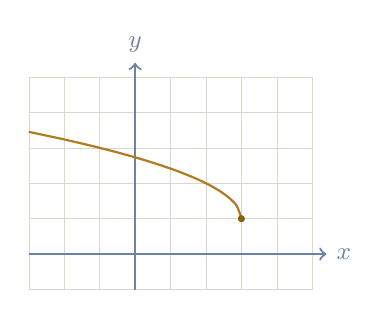
\begin{tikzpicture}[scale=0.45]
  \draw[step=1cm, linec, very thin] (-3,-1) grid (5,5);
  \draw[->, thick, indigosoft] (-3,0) -- (5.4,0) node[right,font=\small]{$x$};
  \draw[->, thick, indigosoft] (0,-1) -- (0,5.4) node[above,font=\small]{$y$};
  \draw[thick, goldc, domain=-3:3, samples=50, smooth] plot(\x,{sqrt(-\x+3)+1});
  \filldraw[goldstrong] (3,1) circle (2.4pt);
\end{tikzpicture}

\vspace{4pt}
\raggedright\textbf{\color{goldstrong}답} \; $-x+3\geq0 \Rightarrow x\leq3$, 정의역 $\{x\mid x\leq3\}$. 근호값 $\geq0$이므로 $y\geq1$, 치역 $\{y\mid y\geq1\}$. $a=-1<0$이므로 $x$가 작아질수록(왼쪽으로 갈수록) $y$가 커지는 방향으로 뻗어나간다.
\end{answerbox}

\vspace{6pt}
\begin{answerbox}
\textbf{문제 4} \quad 정의역이 $\{x\mid x\geq2\}$, 치역이 $\{y\mid y\geq-1\}$이고 점 $(3,1)$을 지나는 무리함수를 $y=\sqrt{a(x-2)}-1$ 꼴로 놓고 식을 구하시오.\\[4pt]
\textbf{\color{goldstrong}답} \; $(3,1)$ 대입: $1=\sqrt{a}-1 \Rightarrow \sqrt a=2 \Rightarrow a=4$. \; $y=\sqrt{4(x-2)}-1=2\sqrt{x-2}-1$
\end{answerbox}

\section{성취수준 (이 차시 범위)}
\begin{tabularx}{\linewidth}{@{}>{\bfseries\color{goldstrong}}p{0.9cm}X@{}}
\toprule
A & 정의역 제한의 원리를 설명하고, 복잡한 무리함수의 정의역·치역을 구하며 그래프 정보로부터 식을 역으로 구성할 수 있다. \\
B & 무리함수의 정의역을 구하고, $y=\sqrt{a(x-p)}+q$의 그래프를 그릴 수 있다. \\
C & 안내에 따라 간단한 무리함수의 정의역을 구할 수 있다. \\
D & 무리함수와 다항함수를 구별할 수 있다. \\
E & 무리식이 무엇인지 안다. \\
\bottomrule
\end{tabularx}

\section{다음 차시}
\begin{calloutbox}
\textbf{중단원·대단원 마무리 (유리함수와 무리함수 / Ⅲ) $\cdot$ 기말 총정리 --- 42차시.} 39$\sim$41차시를 종합 정리하고, 대단원 Ⅲ 전체 및 기말고사 범위를 총점검한다.
\end{calloutbox}
\end{document}
